\chapterimage{./Images/head3.jpg} % Chapter heading image
\chapter{Signals}

\section{Introduction}

\begin{figure}[H]
    \centering
    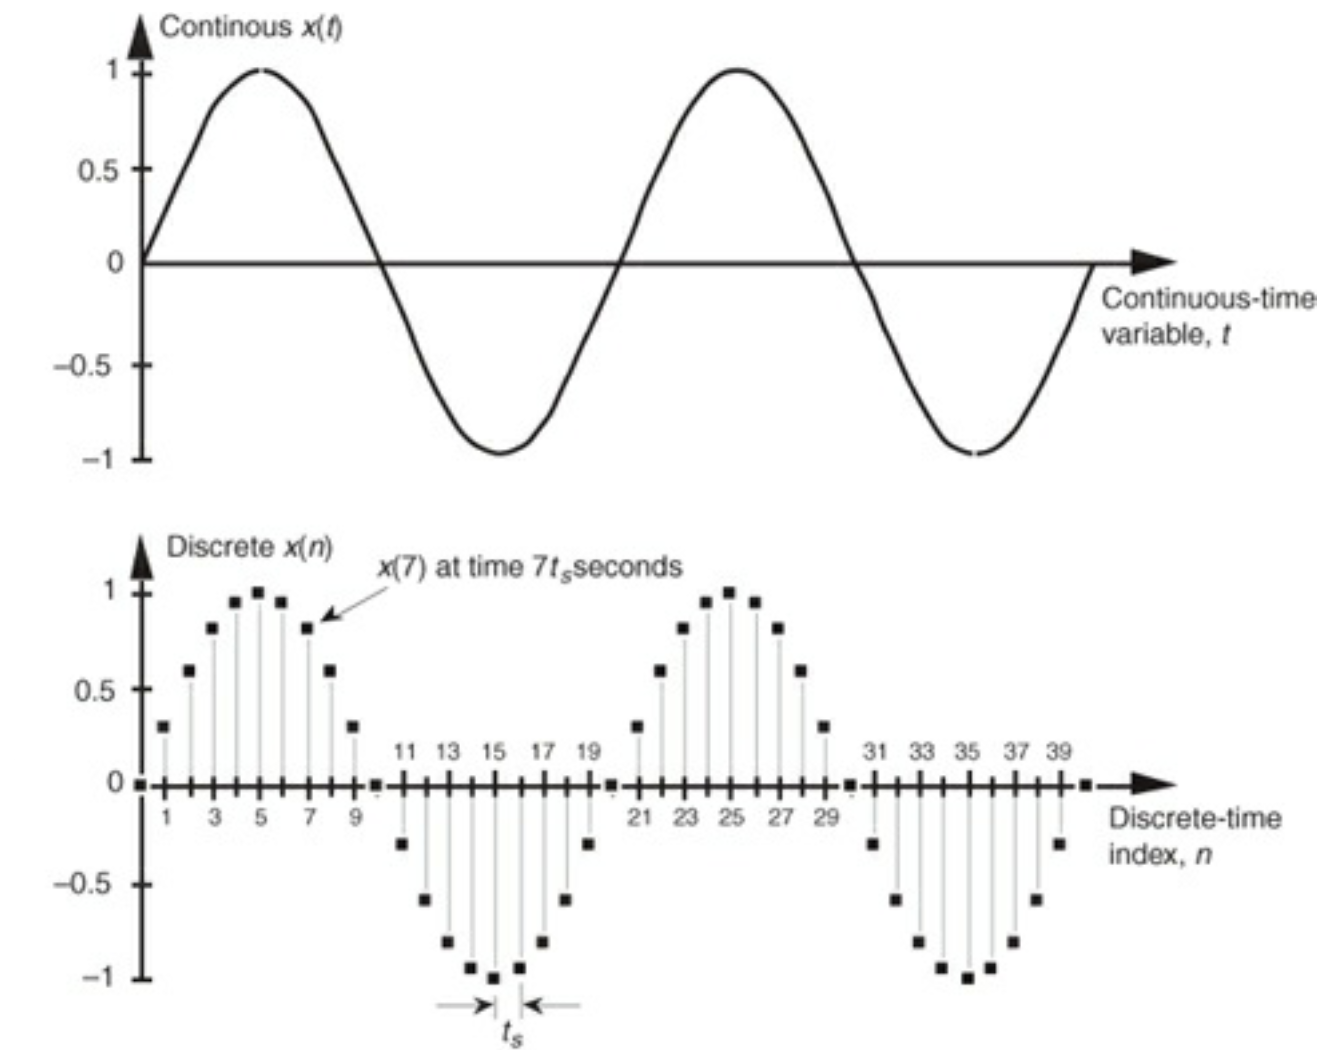
\includegraphics[width=0.5\textwidth]{./LECTURE_2/audio_5.png}
    \caption{Continuous vs. Discrete Signal}
    \label{fig:signal}
\end{figure}

\begin{definition}
    [Important Sets]
    \begin{align*}
        \mathbb{R} & = \text{Set of real numbers}     \\
        \mathbb{Z} & = \text{Set of integers}         \\
        \mathbb{N} & = \text{Set of natural numbers}  \\
        \mathbb{Q} & = \text{Set of rational numbers} \\
        \mathbb{C} & = \begin{aligned}
                           \text{Set of complex numbers} \\
                           \{a+bj : j = \sqrt{-1}\}
                       \end{aligned}
    \end{align*}
\end{definition}

\begin{definition}
    [Conjugate]
    \begin{align*}
        \text{If } z = a + bj, \text{ then } z^* = a - bj
    \end{align*}
\end{definition}

\begin{definition}
    [Magnitude]
    \begin{align*}
        \text{If } z = a + bj, \text{ then } |z| = \sqrt{a^2 + b^2} = \sqrt{z \cdot z^*}
    \end{align*}
\end{definition}

\begin{remark}
    {Containment of Sets}
    \begin{align*}
        \mathbb{N} & \subset \mathbb{Z} \subset \mathbb{Q} \subset \mathbb{R} \subset \mathbb{C}
    \end{align*}
\end{remark}

\begin{definition}
    [Signal]
    A Signal is a function of time.
    \textit{Note: This is not entirely accurate, as we'll see later in the course.}
    \begin{align*}
        x(t) & = \begin{aligned}
                     \text{Continuous signal} \\
                     \text{where } t \in \mathbb{R}
                 \end{aligned} \\
        x[n] & = \begin{aligned}
                     \text{Discrete signal} \\
                     \text{where } n \in \mathbb{Z}
                 \end{aligned}
    \end{align*}
\end{definition}

\begin{definition}
    [Function]
    A function $f:A \to B$ from a set $A$ (the domain) to a set $B$ (the co-domain) is a rule that assigns to each element $a \in A$ exactly one element $b \in B$.
\end{definition}
\begin{example}
    \begin{figure}[h]
        \centering
        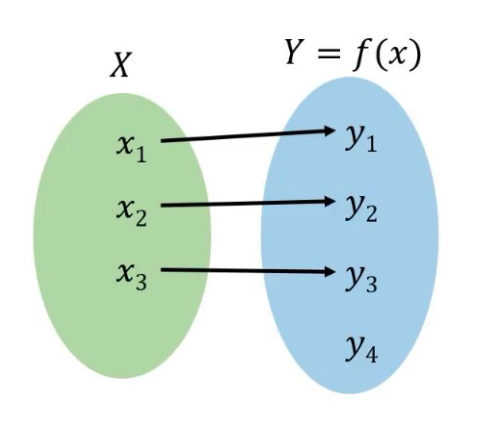
\includegraphics[width=0.5\textwidth]{./LECTURE_2/domain-range-codomain.png}
        \caption{Function}
        \label{fig:function}
    \end{figure}
    Domain of $f$, $A = \{x_1,x_2,x_3\}$, Co-domain of $f$, $B = \{y_1,y_2,y_3,y_4\}$, Range of $f$, $\{y_1,y_2,y_3\}$ (the set that contains all the images of the elements of the domain).
\end{example}

\begin{definition}
    [Range]
    The range or image of a function is the set of all possible values that the function can take. With reference to \ref{fig:function}, the range of $f$ is $\{y_1,y_2,y_3\}$.
\end{definition}

\begin{definition}
    [Inverse Image]
    The inverse image of a subset $C$ of the co-domain of a function $f$ is the set of all elements of the domain that map to the members of $C$. With reference to \ref{fig:function}, the inverse image of $\{y_1,y_2\}$ is $\{x_1,x_2\}$.
\end{definition}

\begin{definition}
    [Injective or One-to-One]
    A function $f:A \to B$ is injective if for every $b \in B$, there is at most one $a \in A$ such that $f(a) = b$. \\
    if $f(a_1) = f(a_2)$, then $a_1 = a_2$ and vice versa.
\end{definition}

\begin{figure}[h]
    \centering
    \begin{tikzpicture}
        % Define the sets
        \node (A1) at (0,3) {$A$};
        \node (A2) at (0,2) {$a_1$};
        \node (A3) at (0,1) {$a_2$};
        \node (A4) at (0,0) {$a_3$};

        \node (B1) at (4,3) {$B$};
        \node (B2) at (4,2) {$b_1$};
        \node (B3) at (4,1) {$b_2$};
        \node (B4) at (4,0) {$b_3$};
        \node (B5) at (4,-1) {$b_4$};

        % Draw arrows
        \draw[->] (A2) -- (B2);
        \draw[->] (A3) -- (B3);
        \draw[->] (A4) -- (B4);

        % Draw sets
        \draw[dashed] (-0.5,3.5) rectangle (0.5,-0.5);
        \draw[dashed] (3.5,3.5) rectangle (4.5,-1.5);
    \end{tikzpicture}
    \caption{Injective (One-to-One) Function}
    \label{fig:injective}
\end{figure}

\begin{definition}
    [Surjective or Onto]
    A function $f:A \to B$ is surjective if for every $b \in B$, there is at least one $a \in A$ such that $f(a) = b$.
    \[
        \forall b \in B, \exists a \in A \text{ such that } f(a) = b
    \]
    % figure

\end{definition}

\begin{figure}[h]
    \centering
    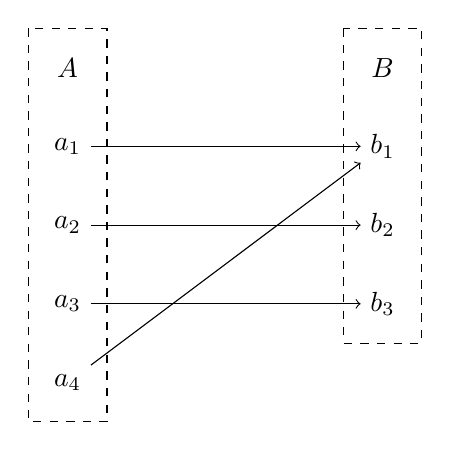
\begin{tikzpicture}
        % Define the sets
        \node (A1) at (0,3) {$A$};
        \node (A2) at (0,2) {$a_1$};
        \node (A3) at (0,1) {$a_2$};
        \node (A4) at (0,0) {$a_3$};
        \node (A5) at (0,-1) {$a_4$};

        \node (B1) at (4,3) {$B$};
        \node (B2) at (4,2) {$b_1$};
        \node (B3) at (4,1) {$b_2$};
        \node (B4) at (4,0) {$b_3$};

        % Draw arrows
        \draw[->] (A2) -- (B2);
        \draw[->] (A3) -- (B3);
        \draw[->] (A4) -- (B4);
        \draw[->] (A5) -- (B2);

        % Draw sets
        \draw[dashed] (-0.5,3.5) rectangle (0.5,-1.5);
        \draw[dashed] (3.5,3.5) rectangle (4.5,-0.5);
    \end{tikzpicture}
    \caption{Surjective (Onto) Function}
    \label{fig:surjective}
\end{figure}

\begin{definition}
    [Bijective]
    A function $f:A \to B$ is bijective if it is both injective and surjective.

\end{definition}
\begin{figure}[h]
    \centering
    \begin{tikzpicture}
        % Define the sets
        \node (A1) at (0,3) {$A$};
        \node (A2) at (0,2) {$a_1$};
        \node (A3) at (0,1) {$a_2$};
        \node (A4) at (0,0) {$a_3$};

        \node (B1) at (4,3) {$B$};
        \node (B2) at (4,2) {$b_1$};
        \node (B3) at (4,1) {$b_2$};
        \node (B4) at (4,0) {$b_3$};

        % Draw arrows
        \draw[->] (A2) -- (B2);
        \draw[->] (A3) -- (B3);
        \draw[->] (A4) -- (B4);

        % Draw sets
        \draw[dashed] (-0.5,3.5) rectangle (0.5,-0.5);
        \draw[dashed] (3.5,3.5) rectangle (4.5,-0.5);
    \end{tikzpicture}
    \caption{Bijective (One-to-One and Onto) Function}
    \label{fig:bijective}
\end{figure}
\end{document}